% DOCX paragraph 364
\chapter{Curving Spacetime}\label{ch:04}

% DOCX paragraph 367
In the previous chapter, we laid the foundations needed to understand some of the
fundamental concepts of Einstein's theory of gravity and, in particular, how his
equations establish a strong and indissoluble link between the curvature of spacetime
and the presence of matter energy. We have also seen that curvature, when present,
changes the state of motion of an object, giving rise to a dynamic that we interpret as
gravity. All this leads us to two questions that can close the line of thought followed
so far: ``How does spacetime actually curve? And how can we measure curvature?''.

% DOCX paragraph 368
Before providing a detailed answer, I would remind you that we have already encountered
two methods by which it is possible, at least in principle, to measure curvature. The
first consists of transporting a vector\index{vector} along a closed circuit while
keeping it parallel to its initial direction; the second method, instead, involves
measuring the deviation of a beam of light from a straight line. While both are valid,
they are not particularly practical or easy to use. We really want a simple and
effective method to get an idea of the strength of the curvature of a given spacetime,
possibly simply by looking at its global properties. In particular, since the curvature
is generally induced by objects with precise \emph{macroscopic} properties (such as mass
and size), it would be useful to have a method based on those properties that provides a
measurement of the curvature produced by the object. In this way, we will not only learn
to measure the degree of curvature, but we will also be able to \emph{produce it!}

% DOCX paragraph 369
However, to get to what we are looking for, it is necessary to take a step back and
return to what we have just discussed. We have said that the curvature radius is a
length-scale associated with the radius of the sphere that approximates the curvature of
spacetime at a given point. This length-scale can differ significantly, depending on
whether we consider the curvature produced by an object with a very small mass (such as
a grain of sand) or a very large mass (such as a supermassive galaxy). Furthermore, this
length-scale can vary locally: it can be enormous if spacetime is almost flat or very
small if it is strongly curved.

% DOCX paragraph 370
To obtain an indicator of curvature that works well for both a grain of sand and a
galaxy, we need a \emph{relative measurement}. In other words, a ratio between two
quantities: one indicating how strong the curvature is (and therefore linked to the
object's mass) and another indicating how it is distributed in space (and therefore
connected to its dimensions). Mathematically, this is a very simple ratio to calculate,
and the Einstein equations are extremely transparent from this point of view. In fact,
they tell us that the \emph{relative strength of spacetime curvature} can be expressed
through the ratio: \index{spacetime!curvature measure}

% DOCX paragraph 373
\begin{equation}\label{eq:04-01}
\begin{gathered}
\begin{pmatrix}\text{relative strength of} \\ \text{spacetime curvature}\end{pmatrix}
\sim \left(\textcolor{gray}{\frac{G}{c^{2}}}\frac{M}{R}\right) \\
= \frac{(\text{mass of an object})}{(\text{size of an object})}
\end{gathered}
\end{equation}

% DOCX paragraph 374
% Equation number is generated with the preceding equation.

% DOCX paragraph 376
In this case, we must also distinguish the parts of the equation that are ``accessory'',
or at any rate unimportant, for the purposes of our discussion (indicated in grey above)
from those that are important mathematically and physically. In Equation \eqref{eq:04-01}, in
particular, the fundamental elements are the mass of the object \emph{(M)} and its
radius \emph{(R)}. Their ratio \emph{M/R} in Equation \eqref{eq:04-01} is also called
\emph{compactness}\index{compactness}. In addition to being a very simple expression and
a convenient tool to measure curvature, Equation \eqref{eq:04-01} shows that to assess an object's
ability to deform spacetime, one should not consider just one aspect (i.e., the mass or
size), but both should be taken into account, as in the definition of compactness. The
greyed-out parts in Equation \eqref{eq:04-01}, that is, the gravitational constant \emph{(G)} and
the speed of light \emph{(c)}, are only necessary for dividing quantities expressed in
different units of measurement. For example, the mass could be in kilograms, and the
radius could, for instance, be in kilometres.\textsuperscript{\hyperlink{note:04-01}{1}}

% DOCX paragraph 377
Hence, we could use Equation \eqref{eq:04-01} to calculate the curvature strength where you are now
as you read this book --- the surface of the Earth. All it requires is to take the mass
of our planet and divide it by its radius, and we find that the
compactness\index{compactness!Earth}, and thus the relative curvature is:

% DOCX paragraph 380
\begin{equation}\label{eq:04-02}
\begin{gathered}
\left(\textcolor{gray}{\frac{G}{c^{2}}}\frac{M_{\oplus}}{R_{\oplus}}\right)
\approx \left(\textcolor{gray}{\frac{G}{c^{2}}}\right)\frac{5.97\times 10^{24}\ \mathrm{kg}}{6372\ \mathrm{km}} \\
\approx 7\times 10^{-10}=0.0000000007
\end{gathered}
\end{equation}

% DOCX paragraph 381
% Equation number is generated with the preceding equation.

% DOCX paragraph 382
I think it is clear to everyone that a number like 0.0000000007 (a seven preceded by
nine zeros) is extremely small. In other words, this simple calculation tells us that on
the surface of the Earth, the relative curvature is essentially zero, so the spacetime
is \emph{locally flat}. \index{spacetime!flat (locally)}\textsuperscript{\hyperlink{note:04-02}{2}}

% DOCX paragraph 383
However simple, this estimate is enlightening: it provides a mathematical ground for
concepts that so far we have discussed only at a conceptual and intuitive level. In
particular, it shows us why our perception\index{perception} of reality is firmly
anchored in a flat spacetime and is, therefore, very far from a perception of reality
that we might acquire in a curved spacetime. In other words, the difficulties we have in
embracing and understanding what happens in a curved spacetime arise from it being so
far removed from our daily experience of an essentially flat spacetime.

% DOCX paragraph 384
To find an analogy, think how difficult it would be for someone who has always lived in
Polynesia to imagine what it means to wake up in a snowstorm. It would be difficult
simply because they have only an abstract idea of that scenario. Likewise, on Earth, we
live in a locally flat spacetime\index{spacetime!flat (Earth)}, which may explain why we are so
surprised and intrigued by the thought that light can propagate along trajectories other
than a straight line: it is a physical process of which we have no direct experience. It
is inconceivable for us, at least on an intuitive level, to think we could see what lies
behind a particular object if we could only capture the rays of light deflected by a
curved spacetime, as shown in Figure 3.8.

% DOCX paragraph 385
Furthermore, the estimate \eqref{eq:04-02} also explains why (with due exceptions) the theory of
general relativity is not really necessary to study physics on our planet. Indeed, this
is so much so that the large majority of the experiments carried out in laboratories
worldwide do not take into account its corrections. For example, when studying
collisions of elementary particles at the international accelerator
CERN\index{CERN} in Geneva, the interpretation of the experiments is carried out
within the theory of special relativity''\index{special relativity}, that is, assuming a
\emph{perfectly} flat spacetime. This is not because spacetime in Switzerland is
\emph{perfectly} flat (indeed, Equation \eqref{eq:04-02} says it is not), but because the
corrections to account for the local curvature are so small and complex that one can
easily do without them.

% DOCX paragraph 386
In short, the theory of Newtonian gravitation is more than sufficient to study and
calculate the effects of gravity on Earth. In fact, for most of what matters on our
planet, the difference between the results it offers and those derived from Einstein's
general relativity is small enough to be reasonably neglected. Therefore, engineers all
over the world can continue to rely on Newton's gravity without any problem and can
build the tallest of skyscrapers.

% DOCX paragraph 389
\section{Curving Time?}\label{sec:04-time}

% DOCX paragraph 391
While it is true that Newton's theory of gravity is sufficient for almost all practical
purposes on Earth, there is an important exception that confirms this rule: the
\emph{global positioning system} (GPS\index{GPS (Global Positioning System)}). This navigation system allows
us to orient ourselves when driving a car or strolling through a city. Without going
into the details of its operation, it is sufficient to recall that the GPS uses a series
of satellites orbiting the planet which communicate continuously with receivers on the
ground, such as our smartphones. The ultimate goal is to use the information gathered
from at least three satellites to \emph{triangulate} our position with a prescribed
precision.

% DOCX paragraph 392
Essential in this triangulation process is the \emph{time of flight}, that is, the time
it takes for the electromagnetic signal to pass from us to the ground stations and then
to the satellites. For an accurate calculation, extremely precise
atomic\index{atomic!clock} clocks are used both on the ground and on satellites, with a
deviation of only 40 nanoseconds per day. That is to say, the time measurements on the
ground stations and on the satellites cannot differ by more than 40 nanoseconds over the
80 trillion nanoseconds that make up a day. We are talking about two parts in a million
million. Despite the tremendous accuracy of these clocks, the GPS would not work without
the corrections that take into account that clocks on satellites and those on Earth
``advance'' with different rates, and these corrections are related to the theory of
general relativity.

% DOCX paragraph 393
To understand why the ``ticking'' of clocks depends on their position, we need to recall
some of the concepts discussed in the previous pages. In particular, within general
relativity, time plays a role similar to that of space. The presence of matter induces
deformations in the elastic fabric of spacetime, changing the relative distances between
its points, i.e., between events.

% DOCX paragraph 394
Hence, just as the bowling ball affects the separation between different areas of the
sheet (i.e., the distance between the points of a \emph{spatial
section}\index{section!spatial} of spacetime in which events all have the same time), so the
presence of matter affects the separation between different instants of time (i.e., the
distance between the points of a \emph{temporal section}\index{section!temporal} of spacetime
in which all events have the same position).

% DOCX paragraph 395
Indeed, if you think about it, we use clocks and watches to precisely measure the
separation in time between two events. This can be done by exploiting different
technologies: the small rotation of a gear to which the hand of a watch is connected (if
it is analogue) or the oscillation of an electron between two precise energy states in
an excited atom (if it is an atomic clock). In both cases, however, we expect the
ticking rate, for example, of two identical Swiss chronograph watches, to be the same
everywhere, in Zurich and New York. However, according to general relativity, this is
only possible in one case: if they are stationary and within a flat spacetime. If,
conversely, they are in motion, then even in a flat spacetime there will be a
dilation\index{time dilation} of time, as predicted by the theory of special
relativity''\index{special relativity} and verified every day in particle accelerators such as
that at CERN\index{CERN}. Furthermore, if spacetime is curved, as expected in the
presence of matter, then the rate of advancement will also depend on the position: the
same Swiss chronograph will mark time differently in Zurich and New York. This
difference is due to Zurich being located at an altitude of 408 metres above sea level
and, therefore, within a slightly weaker gravitational field than that of New York,
which is only 10 metres above sea level.

% DOCX paragraph 396
In other words, according to general relativity\index{general relativity} (and its idea of an
elastically deformable spacetime), it is perfectly natural that time is as flexible as
space, and both can be curved. Equally natural is that the advancement of time is a
function of the position, precisely because curvature generally changes from place to
place, as shown in Figure 3.5. There, our sheet was almost flat at the edges, while it
exhibited a very marked curvature near the bowling ball.

% DOCX paragraph 397
The change in the advancement of time in the presence of a curved spacetime also takes
the name \emph{time dilation}\index{time dilation}. General relativity quantifies with
great precision this dilation\index{time dilation} on the basis of different degrees of
curvature. We will return to this concept in Chapter 6 when we deal in more detail with
the dilation\index{time dilation} of time that occurs in the vicinity of a black hole.
However, for the time being, I would like to affirm what general relativity predicts. In
an area of spacetime with a marked curvature (therefore within a stronger gravitational
field), time flows ``more slowly'' than in an area with less curvature (therefore in a
weaker gravitational field).

% DOCX paragraph 398
\begin{figure}[htbp]
\centering
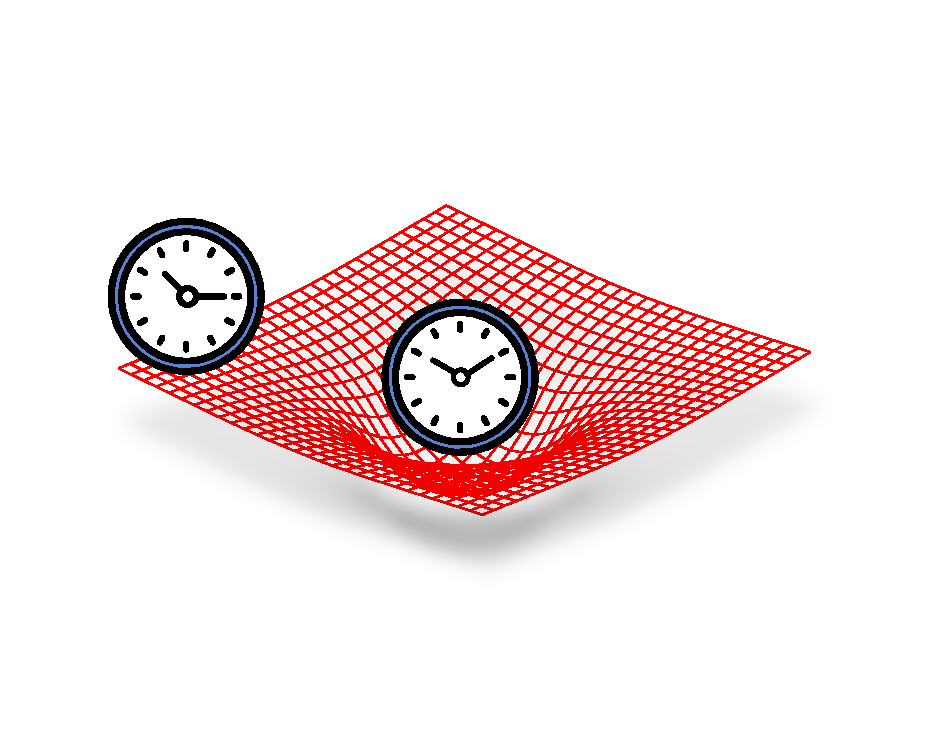
\includegraphics[trim=43bp 72bp 45bp 94bp,clip,width=0.88\linewidth,height=0.48\textheight,keepaspectratio]{../figs/pdf/en/fig-04-01.pdf}

% DOCX paragraph 400
\caption{\emph{The rate of advancement of clocks depends on the curvature of spacetime
and, therefore, on their position. Those in a nearly flat area of spacetime will go
faster than their counterparts located in a highly curved area.}}\label{fig:04-01}
\end{figure}

% DOCX paragraph 402
To return to the GPS, this means that the clocks in the stations on Earth, where the
curvature and gravity are greater, will accumulate a delay of about 45 microseconds
(i.e., 45,000 nanoseconds) per day compared to identical clocks placed on the satellites
in orbit at 20,000 kilometres from the Earth's surface, where curvature and gravity are
smaller. This time difference is far greater than the maximum acceptable for the correct
functioning of the GPS, that is, 40 nanoseconds per day. Therefore, without an
appropriate calibration of the clocks, the GPS would provide completely incorrect
information on our position.

% DOCX paragraph 403
I realise that all this may sound incredible or even absurd: I, too, have to summon up
all my imagination to accept a phenomenon so alien to our perception\index{perception}
of reality. However, luckily for us, what I have illustrated to you no longer represents
the abstruse consequence of a bizarre theory: it is a precise prediction that today we
can verify experimentally! Indeed, as science fiction-like as it may sound, we are now
able to accurately measure the difference in the ticking rate of atomic clocks that are
simply placed on different floors of an ordinary building. The ability to perform such
measurements has allowed us to confirm what Einstein predicted more than a hundred years
ago: a clock placed on the first floor of a building, and therefore within a stronger
gravitational field, will lag behind its identical counterpart on the second floor,
where the field is weaker. As you can easily imagine, the difference is minuscule! So,
don't try using it as an excuse for being late for an appointment --- just because your
watch was in a place with a high spacetime curvature~...

% DOCX paragraph 406
\section{In Search Of Strong Curvature}\label{sec:04-search}

% DOCX paragraph 408
Let us now return to the estimate of curvature given by Equation \eqref{eq:04-01}. We have
established that curvature is almost zero on our planet, but we can still go and ``look
for'' a more severe curvature in our neighbourhood, say, within the solar system. So,
let us imagine building a device to measure relative curvature and hopping from planet
to planet to see how the measured values change. What would we discover? First of all,
in interplanetary space, where there is very little matter, the curvature is even
smaller than on Earth, and therefore spacetime is even flatter there! Curvature would
become perceptible only when we get closer to a planet, but it would still have values
comparable to those we have seen for the Earth. Then, as we continue our journey within
the solar system, the device would reveal that the maximum value is actually reached on
the surface of our star.

% DOCX paragraph 409
To know the compactness of the
Sun\index{Sun!curvature}\index{Sun!compactness}\index{Sun!mass}\index{Sun!radius}, we just
have to use the Equation \eqref{eq:04-02}, substituting its mass and its radius for those of the
Earth.

% DOCX paragraph 411
\begin{equation}\label{eq:04-03}
\begin{gathered}
\left(\textcolor{gray}{\frac{G}{c^{2}}}\frac{M_{\odot}}{R_{\odot}}\right)
\approx \left(\textcolor{gray}{\frac{G}{c^{2}}}\right)\frac{1.98\times 10^{30}\ \mathrm{kg}}{695\,000\ \mathrm{km}} \\
\approx 2\times 10^{-6}=0.000002
\end{gathered}
\end{equation}

% DOCX paragraph 412
% Equation number is generated with the preceding equation.

% DOCX paragraph 413
As we can see, the Sun's compactness\index{compactness!Sun} is about three thousand times
larger than that of the Earth and equal to 0.000002, or two parts in a million. As a
result, the curvature of spacetime near our star is greater than that which we
experience on our planet. This is because the mass of the Sun is three hundred thousand
times that of the Earth, but its radius is only a hundred times larger. Hence, with
regard to the Sun, although the denominator in the ratio \emph{M/R} is larger than for
the Earth, the numerator increases even more. However, in this case, we still obtain a
disappointingly small value of curvature, so small that if we were to represent it
visually through the deformation of a sheet, it would still appear flat even to those of
us with the best eyesight.

% DOCX paragraph 414
Of course, if we could directly experience its effects, the curvature of spacetime near
the Sun would still be sufficient to produce perceptible variations in our daily
experience. In fact, the gravitational field would be about 28 times larger there; for
example, assuming that on Earth you weigh about 70 kilograms, the same scale
hypothetically placed on the surface of the Sun would tell you that now, weighing 2,000
kilos, you are terribly ``overweight''! In reality, your body mass would not have
changed at all --- you could always make up for this by weighing yourself on the
Moon\index{Moon}, thus discovering you have ``lost weight'', as the scale there
would measure a weight of only 12 kilos. Similarly, on the Sun's surface, the
differences between clocks placed in configurations similar to those of the GPS would be
of the order of hundredths of a second per day. This is an amount of time that we all
have a precise idea of (think how much we use it in racing sports).

% DOCX paragraph 415
By calculating the compactness as given by Equation \eqref{eq:04-01}, we can easily determine the
relative curvature produced by any object, which can lead us to surprising and otherwise
unexpected conclusions. Let us take, for example, two very different objects: a star
like the Sun and a galaxy like our own Milky\index{Milky Way} Way. Well, the first has
a mass of 1,000 billion billion billion kilograms (or, more simply,
10\textsuperscript{30} kilograms): a value that in astronomy is used as a unit of
reference and is called the \emph{solar mass}. The second object has a mass equal to
about 1,000 billion solar masses, a number that corresponds more or less to the number
of stars it contains. Such information could lead us to conclude that it produces a
proportionately more severe curvature since the Milky\index{Milky Way} Way has a mass
considerably greater than that of the Sun. In reality, this is not the case; it is
enough to compare the compactness of the two objects to realise this and understand why.
In particular, the radius of the Sun is of the order of 700,000 kilometres, while that
of our galaxy is approximately equal to 16,000 \emph{parsecs} (which is about 53,000
light years, that is, 10\textsuperscript{17} kilometres).\textsuperscript{\hyperlink{note:04-03}{3}} Now, if we
compute the compactness\index{compactness!Milky Way} \emph{M/R} of the Milky\index{Milky Way}
Way, we would realise that it is comparable to that of the Sun, namely, of the order of
some parts in a million (to be precise, \emph{M/R} ≃1.80 × 10\textsuperscript{--6}). The
reason is obvious: our galaxy is considerably more massive but also much more extended
and diluted, so its compactness does not differ much from that of the Sun. In short, the
curvature produced by these two radically different objects, and hence the curvature
radius, is almost the same. So, if we were aboard a spacecraft and approached either one
from very far away (i.e., if our spacecraft acted as what is technically called a
\emph{test particle}\index{test particle}), we would experience essentially the same
gravitational field and would have to change our trajectory using the same amount of
fuel.

% DOCX paragraph 416
This example warns us of a common mistake made when thinking of curvature. In
particular, when considering the curvature produced by an object, it is misleading to
focus only on its mass or its size, as both quantities provide us with only a partial
view. On the contrary, the ratio between these two quantities informs us how much mass
\emph{M} is confined in a certain region of spacetime of size \emph{R} to produce a
relative curvature proportional to \emph{M/R}.

% DOCX paragraph 417
Finally, the estimates for the compactness of the Earth \eqref{eq:04-02} and of the Sun \eqref{eq:04-03} can
help us to learn an important lesson. In both cases, extremely small numbers correspond
to very modest curvatures and generate equally small changes in the dynamics of objects
that move near these bodies. In other words, the compactness of the Earth and that of
the Sun clearly tells us that although spacetime is in principle \emph{elastic}, it is
nevertheless very \emph{rigid}. Basically, the sheet in our example is quite hard to
bend!

% DOCX paragraph 418
This conclusion appears almost disarming as it would seem to indicate that Einstein's
theory of general relativity is fundamentally useless. Indeed, the theory focuses on
what happens when the curvature is large, but all our estimates tell us the curvature is
almost always zero or so small that it can be neglected, as in the experiments at
CERN\index{CERN}.

% DOCX paragraph 421
\section{A Theory Nobody Liked ...}\label{sec:04-history}

% DOCX paragraph 423
What has been illustrated so far, particularly the consideration that spacetime is very
hard to bend, gives us a better understanding of the historical development and the
early impact of general relativity\index{general relativity} within modern physics. It helps us
to appreciate why no one really liked this theory, except for the few who understood it
in detail and were fascinated by it. The latter includes the aforementioned Sir Arthur
Eddington\index{Eddington, Sir Arthur}, an arduous defender of the theory, who introduced it to
the British scientific community. A community that was not very sympathetic to the ideas
of a German scientist (don't forget these were the years of the First World War and the
period immediately thereafter).

% DOCX paragraph 424
When proposed, numerous scientists (even famous ones) strongly opposed the theory of
general relativity. This attitude towards Einstein's innovative ideas --- a rejection
that began long before, with the publication of the theory of special
relativity''\index{special relativity} --- had different roots, some even very deep. To begin
with, the mathematical aspects of the theory were so complex that only few were able to
follow them in detail and understand their consequences. An illuminating anecdote brings
us back to Eddington\index{Eddington, Sir Arthur}'s presentation of the results of measurements of
the deflection of light during the total solar eclipse\index{solar eclipse} of 1919. It is
said that a reporter asked Eddington\index{Eddington, Sir Arthur} if it were true that only three
people in the world were able to understand general relativity\index{general relativity}. To
which he jokingly replied: ``Oh, really? And who would be the third?''.

% DOCX paragraph 425
The attitude of rejection towards Einstein's new theory was largely due to the fact that
it proposed a radically different view of gravity, in which purely mathematical and
geometric considerations (namely, spacetime curvature) could actually explain what was
perceived as a purely physical interaction.

% DOCX paragraph 426
In addition, the main character of this new theory (curvature) is always essentially
zero, at least as far as it was experimentally measurable in those times, so it was
unclear precisely what impact it could have in practice. Finally, to make the picture
even more discouraging, the theory implied apparently paradoxical or even absurd
consequences, such as time dilation\index{time dilation} or length contraction.

% DOCX paragraph 427
Many of these objections, and the openly hostile attitude of numerous scholars, were
overcome when two of the theory's predictions, namely, the bending of light and
Mercury's perihelion\index{perihelion} precession, were confirmed experimentally.
However, these successes only changed the ``formal'' attitude of the scientific
community towards general relativity, but not the factual one. Many physicists continued
to consider it (and to some extent continue to do so today) as a theory which, although
not incorrect, remained of little use for practical purposes, applicable to physical
conditions of curvature very different from those typically encountered in nature.

% DOCX paragraph 428
Thus, for decades, general relativity was a theory of interest primarily for
mathematicians, who appreciated its rich structure and geometric elegance. On the other
hand, physicists remained perplexed by the bizarre predictions and somewhat disarmed by
the complexities of the equations, which often remained unsolvable, except for a few
simple and idealised cases. Furthermore, given the physical conditions for which it was
relevant (that were very distant from conditions usually encountered in labs and
experiments), general relativity was accepted not so much because it was correct and
important but rather because it was fundamentally irrelevant. In other words, Newton's
theory of gravitation, however inaccurate, was simpler to use and remained accurate
enough to be the only theory needed for all practical purposes.

% DOCX paragraph 429
For decades, this attitude of scepticism condemned general relativity to a state of
effective neglect, denying it the development it deserved and which it would only come
to know many years later. Indeed, a newly-formulated theory can only offer a vague idea
of the conceptual and experimental implications it can express when fully developed. To
explore such implications in detail, the collective effort of the entire scientific
community is necessary, which (often in no particular order) delves into the dark
meanderings of the theory and gradually illuminates and reveals its various aspects.
Unfortunately, none of this happened for the theory of general relativity. Between 1916
(the year of its publication) and the beginning of the 1960s, it remained the
prerogative of a small group of interested physicists and mathematicians.

% DOCX paragraph 430
The turning point, and what could be considered as the ``Renaissance'' of general
relativity\index{general relativity}, came when new and surprising astronomical observations
(in particular taken by satellites sensitive to X-ray\index{X-ray!radiation} radiation)
\index{radiation!X-ray} began to provide overwhelming evidence concerning the existence of
compact celestial objects whose phenomenology was inexplicable within a Newtonian
gravitational framework. The incontrovertible evidence that extremely compact objects
existed and were capable of releasing enormous amounts of energy forced the scientific
community to reconsider the ``bizarre solutions'' envisaged by general relativity almost
fifty years earlier.

% DOCX paragraph 431
Einstein's revenge came when nature itself showed us that, although spacetime is nearly
flat within the solar system, there are portions of the universe where it is not so at
all. Moreover, astronomical observations have revealed regions of the cosmos where
nature is able to overcome the enormous rigidity of spacetime, producing high curvatures
that can even become extreme, as in the case of black holes. Under similar conditions,
general relativity provides a mathematically adequate framework and becomes the only
theory capable of explaining --- with enormous success --- the functioning of the
physical world.

% DOCX paragraph 432
In Chapters 5 and 6, we will consider two of the most striking examples of extreme
curvature nature can produce, namely neutron stars and black holes. Now, however, a
final consideration awaits us.

% DOCX paragraph 435
\section{A Gedanken Experiment}\label{sec:04-experiment}

% DOCX paragraph 437
Before closing this chapter, I would like to invite you to perform what Einstein liked
to call a \emph{gedanken experiment}, that is, a ``thought experiment'' conducted
through imagination alone. I recall that, in general, an experiment is aimed at
ascertaining whether a certain phenomenon occurs as predicted by the theory under very
precise and reproducible conditions. To carry out the experiment typically requires a
laboratory, an accelerator, or instruments such as a satellite or telescope. In this
sense, a gedanken experiment is something decidedly anomalous; in fact, it does not
require any experimental apparatus. Instead, it is conducted by engaging only our minds
on the basis of logical and physical considerations that allow us to obtain ``virtual''
results that would be very difficult to produce in a real laboratory. In other words, a
thought experiment is another way to find answers to questions like: ``What would happen
if~...?''. Therefore, all we need to conduct a gedanken experiment is a good dose of
imagination and an excellent knowledge of physics. If you provide the first component, I
will help with the second so that together we can carry out a gedanken experiment to
investigate the limits of gravity.

% DOCX paragraph 438
So, let us start from Equation \eqref{eq:04-01} to measure the compactness of an object. We said
that the higher its value, the higher the relative rate of curvature. Since the
compactness is given by the ratio between the mass, \emph{M}, and the size of an object,
\emph{R}, we can increase the value of the ratio \emph{M/R} by keeping the numerator
constant and progressively reducing the denominator. From a physical point of view, we
can do this in practice by taking an object, for example, a star like the Sun, and
compressing it progressively to reduce its radius. Imagine a huge press that
``squeezes'' the Sun more and more and reduces its radius following our wishes --- I
admit you need some imagination here, but this is what gedanken experiments are all
about! The result of the process is shown schematically in Figure \ref{fig:04-02}, and we can
analyse it together.

% DOCX paragraph 439
More specifically, the panel on the left reports the spacetime curvature when we have
reduced the radius of the Sun from its initial 700,000 kilometres to about 15, that is,
the size of a moderately large city. Thus, the compactness \emph{M/R} has increased
dramatically, from the order of two-millionths of the estimate \eqref{eq:04-03} to 0.1, i.e., to
about 10\%\index{compactness!compact star}. Here, we can see that the deformation of the surface is
visible to the naked eye, even without the aid of a greyscale (in all of the three
squares of Figure \ref{fig:04-02}, the ``sheet'' has a length of 60 kilometres). In particular, note
that the surface undergoes almost no deformation in the areas farthest from the centre,
i.e., at the corners, indicating that spacetime is still essentially
flat\index{spacetime!flat (nearly)}\index{spacetime!curved} in those regions. In the centre, however, the
curvature is clearly visible and has the smooth shape of a bowl.

% DOCX paragraph 442
\begin{figure}[htbp]
\centering
\[\begin{array}{@{}w{c}{0.2933\linewidth}@{}w{c}{0.2933\linewidth}@{}w{c}{0.2933\linewidth}@{}} R_{\odot}\cong15\ \mathrm{km} & R_{\odot}\cong7.5\ \mathrm{km} & R_{\odot}\cong5\ \mathrm{km}\end{array}\]

% DOCX paragraph 444
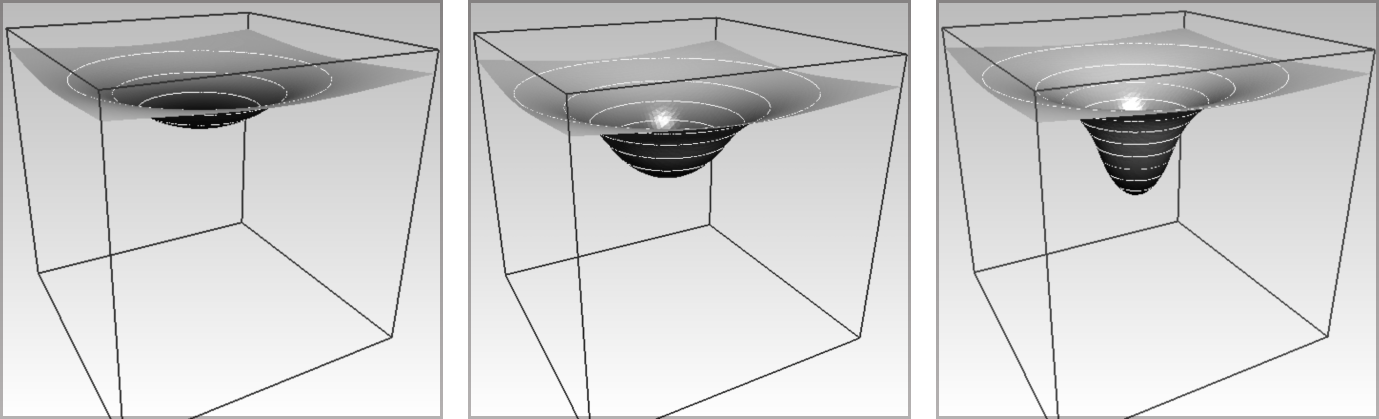
\includegraphics[width=0.88\linewidth,height=0.48\textheight,keepaspectratio]{../figs/pdf/en/fig-04-02.pdf}

% DOCX paragraph 446
\[\begin{array}{@{}w{c}{0.2933\linewidth}@{}w{c}{0.2933\linewidth}@{}w{c}{0.2933\linewidth}@{}} M/R\cong0.1 & M/R\cong0.2 & M/R\cong0.3\end{array}\]

% DOCX paragraph 447
\caption{\emph{A gedanken experiment on the curvature of spacetime produced by the Sun
when its radius is reduced to the value indicated above each square, but its mass
remains unchanged. The relative M/R compactness is indicated below each image.}}\label{fig:04-02}
\end{figure}

% DOCX paragraph 449
The panel in the middle of Figure \ref{fig:04-02}, on the other hand, shows what would happen if we
continued our shrinking process and further shrunk the Sun to obtain a radius of about
7.5 kilometres, thus halving its size when compared to that in the previous box. In this
case, the compactness \emph{M/R} would increase to 0.2, that is to say, to around 20\%.
Under these conditions, the curvature becomes even more marked, and the ``bowl''
produced in the sheet becomes much deeper. We can end our gedanken experiment with the
panel on the right in Figure \ref{fig:04-02}, where the Sun has been compressed to a radius of only
5 kilometres. In this case, the compactness \emph{M/R} is about 0.3, or 30\%. The
curvature is very prominent under these conditions, and our sheet, which we had found to
be quite stiff, has now been deformed enormously. What was a simple bowl in the left
panel has become very steep-sided, resembling something that is often referred to as a
``throat\index{throat}''.

% DOCX paragraph 450
It is interesting to note that the degree of curvature in the right panel of Figure \ref{fig:04-02}
is much more severe than that in the left panel, although when moving from one to the
other, we have reduced the size of our star by only a third. This is because the
curvature depends, in a nonlinear manner, on the ratio between mass and radius. Under
the appropriate conditions, even a slight variation of \emph{R} can lead to enormous
changes in the curvature. As you can easily imagine by observing the image on the right,
in conditions of curvature of this type, new physical phenomena can occur (and can be
measured through experiments) that are very different from those typically encountered
in a flat spacetime. We will go on to explore and explain such phenomena in due course.

% DOCX paragraph 451
I would like to close this chapter with a few questions that I hope will fuel your
curiosity. We have seen what happens to the curvature of spacetime produced by the Sun
when the star is reduced to a radius of just five kilometres. However, we could ask
ourselves: ``\emph{Is there a limit to how much we can compress an object like the Sun?
If so, what is this limit?}''. And, to continue along this line of thought: ``\emph{If
this limit does exist, can it be overcome? And what would happen if it could be?}''.

% DOCX paragraph 452
We will find answers to these questions on the next leg of our journey.
